% intro.tex:

\chapter{INTRODUCTION} % all caps please
\label{chap:intro}


%multi figure image
\begin{figure}
	\begin{center}
	\subfigure[]{\label{fig:mammography_top}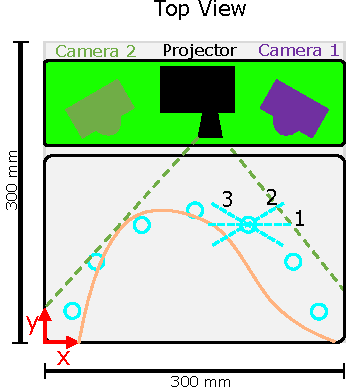
\includegraphics[height=5cm]{mammography_top.pdf}}
	\subfigure[]{\label{fig:mammography_side}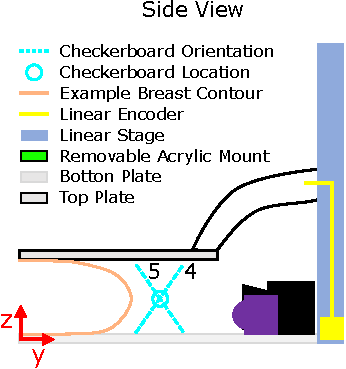
\includegraphics[height=5cm]{mammography_side.pdf}}
	\subfigure[]{\label{fig:mammography_setup}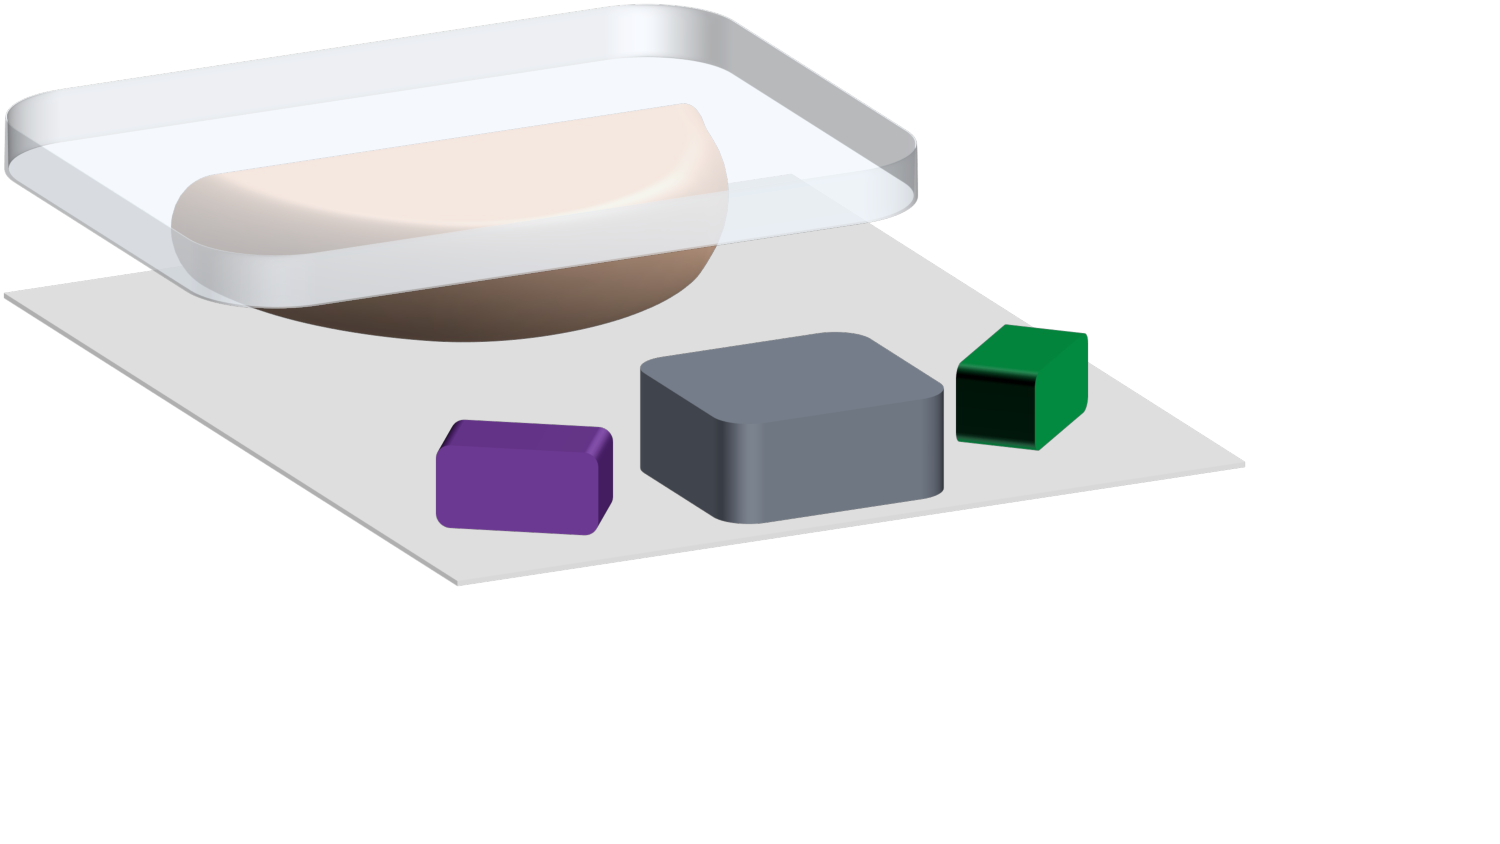
\includegraphics[width=5cm]{sli_model.pdf}}
	\end{center}
	\caption{ (a) Top-view of the breast compression compartment -- upper: SLI system; bottom: horizontal cross-section (orange line) of the compressed breast with blue circles indicating the placement of the checkerboard used for system calibration. Numbers 1-5 indicate the 5 board orientations repeated at each location for calibration. (b) Side-view of the breast compression plates, showing the linear translation stage (blue bar on the right) and a linear encoder (in yellow), and  (c) 3-D rendering of the SLI system, an acrylic bottom plate and an acrylic compression paddle (top). } 
	\label{fig:mammographysetup}
\end{figure} 


% single figure image
\begin{figure}
    \begin{center}
    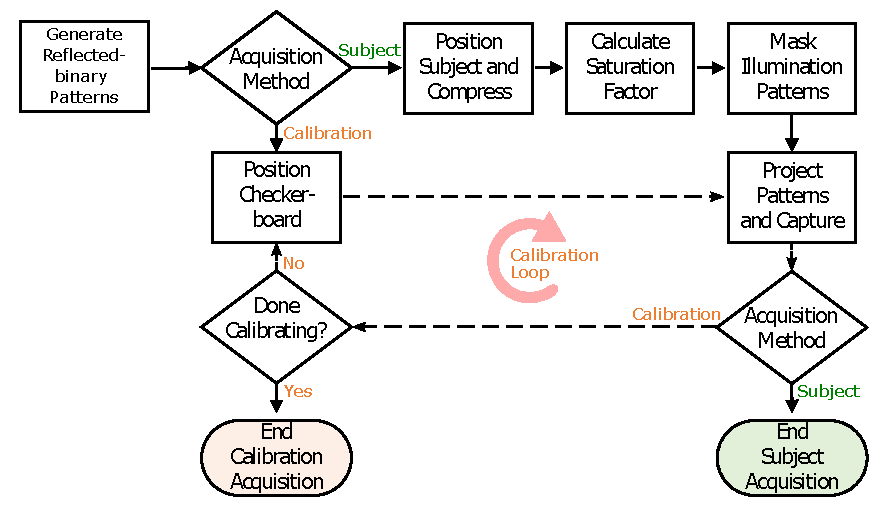
\includegraphics[width=.9\textwidth]{sli_flowchart.pdf}
    \end{center}
    \caption{Flow chart of image acquisition for both subject measurements and system calibration. Subject measurements calculate a saturation scaling factor and mask the illumination patterns prior to projecting patterns. System calibration measurements do not mask the illumination patterns and project at full intensity. The calibration loop (dashed lines) is repeated for each location and orientation of the calibration checkerboard.} 
    \label{fig:sli_flowchart}
\end{figure} 



\section{Life, Universe and Everything}
\label{chap:intro:design}






% --- EOF ---
